\pagebreak
\section{koncepcja snake-a} %Jakub Grzyb
\label{sec:Grzyb}

Grafika koncepcyjna snake-a w konsoli (see Figure~\ref{fig:snake}).

\begin{figure}[hthp] % ustawia obraz w pożadanej pozycji
    \centering
    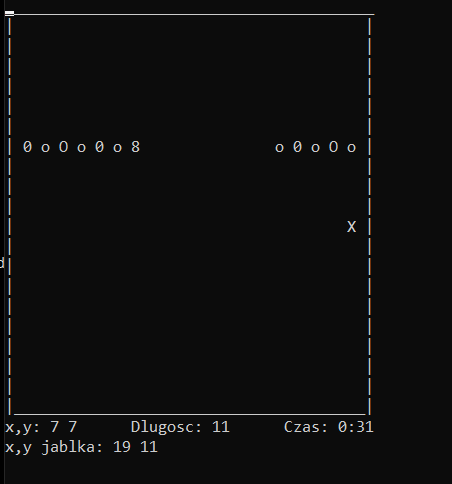
\includegraphics[width=0.4\textwidth]{pictures/snake.png} %Zwiększyć jego "width"
    \caption{Grafika koncepcyjna snake-a w konsoli}
    \label{fig:snake}
\end{figure}

Tabela~\ref{tab:snake} planszy snake-a %pokazuje wartość label czyli numer np tabeli itd

\begin{table}[htbp]
\centering
\begin{tabular}{|l|l|l|}
\hline
\rowcolor[HTML]{675643} 
S & N & A \\ \hline
K & E & C          \\ \hline
O & O & L          \\ \hline

\end{tabular}
\label{tab:snake}
\caption{Caption of my table is below it.}
\end{table}

Dlaczego kompilator umieszcza ten tekst przed obrazkami jeżeli w kodzie jest po?

\begin{itemize}
  \item nie
  \item numerowana
  \item lista 
  \item słów
  \item edytcja

\end{itemize}
\pagebreak

\begin{enumerate}
    \item uno
    \item dos
    \item tres
    \item cuatro
    \item piec
\end{enumerate}

\vspace{4pt}

Wszystko dziala jak trzeba :)
\vspace{6pt}

$c=\sqrt{a^2+b^2}=\frac{P*2}{h}$
\vspace{10pt}

\textbf{Etiam dapibus lacus quis iaculis} \textit{vestibulum. Pellentesque vel maximus diam, nec } \underline{vestibulum} Pellentesque \textbf{vel maximus \emph{diam, nec} tempus magna. Aenean quis scelerisque nibh}. Sed vitae sapien maximus, tristique dolor non, gravida magna. Morbi sed mi nec neque finibus aliquet a nec nisl. Vestibulum nec massa vitae magna tincidunt eleifend ut eu nibh. Ut sodales quis libero eu finibus.

\begin{flushright} Praesent ac ipsum elit. Suspendisse ut lacinia ligula. Quisque pellentesque \textbf{table \ref{tab:snake}} vehicula pulvinar. Nunc molestie iaculis tortor \textit{eget consequat. Aliquam sed}  erat vitae urna sollicitudin vestibulum. Aliquam euismod lorem at nisl feugiat efficitur. \textbf{Nam ut ex sed}  \end{flushright} \begin{center} \textbf{ligula volutpat iaculis} . Cras sed eleifend justo. Class aptent taciti sociosqu ad litora torquent per conubia nostra, per inceptos himenaeos. Proin feugiat, nulla sed lacinia pharetra,  mauris justo lobortis lorem, eget \end{center} laoreet diam erat eget sapien.
